\section{Appendix: Qubit Scaling Trend}

\begin{figure}[H]
\centering
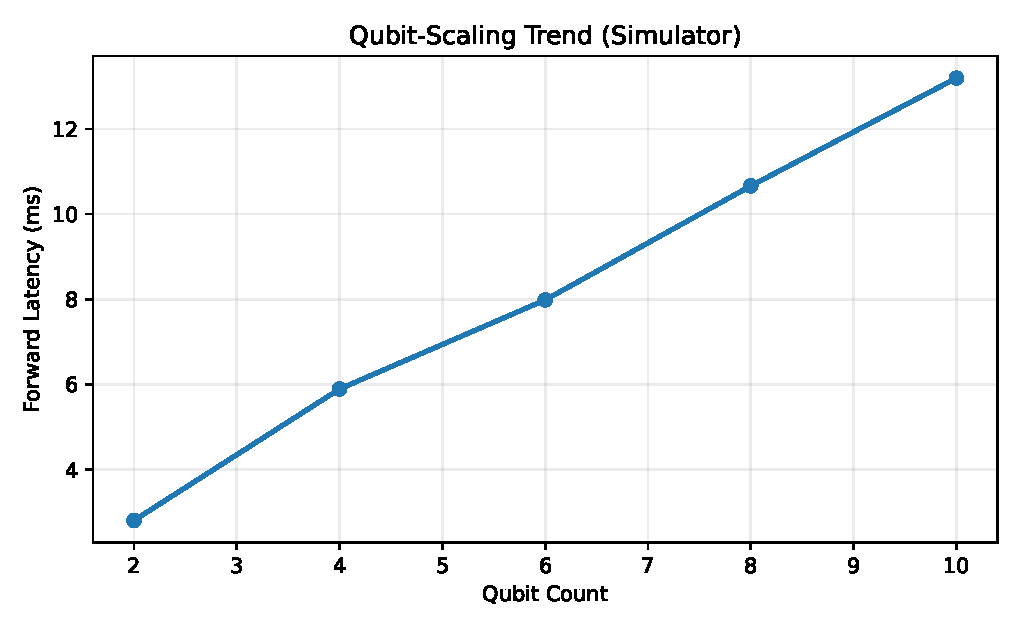
\includegraphics[width=0.78\linewidth]{figures/qubit_scaling_trend.pdf}
\caption{Simulator forward-pass latency versus qubit count (fixed layer depth).}
\label{fig:qubit-scaling-trend}
\end{figure}

\begin{table}[H]
\centering
\footnotesize
\setlength{\tabcolsep}{6pt}
\begin{tabular}{ccccc}
\toprule
Qubits & Layers & Params & $2^n$ State Dim & Forward Latency (ms) \\
\midrule
2 & 4 & 8 & 4 & 2.8066 \\
4 & 4 & 16 & 16 & 5.8931 \\
6 & 4 & 24 & 64 & 7.9832 \\
8 & 4 & 32 & 256 & 10.6610 \\
10 & 4 & 40 & 1024 & 13.1908 \\
\bottomrule
\end{tabular}

\caption{Qubit-scaling simulation summary with state-space growth and measured latency.}
\label{tab:qubit-scaling-trend}
\end{table}

Latency vs qubit count at fixed depth slopes upward---expected, but the slope is why the main body sticks to six qubits: classical simulation budgets mean wire count is not pretend-free.
